% Options for packages loaded elsewhere
\PassOptionsToPackage{unicode}{hyperref}
\PassOptionsToPackage{hyphens}{url}
%
\documentclass[
]{article}
\usepackage{amsmath,amssymb}
\usepackage{iftex}
\ifPDFTeX
  \usepackage[T1]{fontenc}
  \usepackage[utf8]{inputenc}
  \usepackage{textcomp} % provide euro and other symbols
\else % if luatex or xetex
  \usepackage{unicode-math} % this also loads fontspec
  \defaultfontfeatures{Scale=MatchLowercase}
  \defaultfontfeatures[\rmfamily]{Ligatures=TeX,Scale=1}
\fi
\usepackage{lmodern}
\ifPDFTeX\else
  % xetex/luatex font selection
\fi
% Use upquote if available, for straight quotes in verbatim environments
\IfFileExists{upquote.sty}{\usepackage{upquote}}{}
\IfFileExists{microtype.sty}{% use microtype if available
  \usepackage[]{microtype}
  \UseMicrotypeSet[protrusion]{basicmath} % disable protrusion for tt fonts
}{}
\makeatletter
\@ifundefined{KOMAClassName}{% if non-KOMA class
  \IfFileExists{parskip.sty}{%
    \usepackage{parskip}
  }{% else
    \setlength{\parindent}{0pt}
    \setlength{\parskip}{6pt plus 2pt minus 1pt}}
}{% if KOMA class
  \KOMAoptions{parskip=half}}
\makeatother
\usepackage{xcolor}
\usepackage[margin=1in]{geometry}
\usepackage{color}
\usepackage{fancyvrb}
\newcommand{\VerbBar}{|}
\newcommand{\VERB}{\Verb[commandchars=\\\{\}]}
\DefineVerbatimEnvironment{Highlighting}{Verbatim}{commandchars=\\\{\}}
% Add ',fontsize=\small' for more characters per line
\usepackage{framed}
\definecolor{shadecolor}{RGB}{248,248,248}
\newenvironment{Shaded}{\begin{snugshade}}{\end{snugshade}}
\newcommand{\AlertTok}[1]{\textcolor[rgb]{0.94,0.16,0.16}{#1}}
\newcommand{\AnnotationTok}[1]{\textcolor[rgb]{0.56,0.35,0.01}{\textbf{\textit{#1}}}}
\newcommand{\AttributeTok}[1]{\textcolor[rgb]{0.13,0.29,0.53}{#1}}
\newcommand{\BaseNTok}[1]{\textcolor[rgb]{0.00,0.00,0.81}{#1}}
\newcommand{\BuiltInTok}[1]{#1}
\newcommand{\CharTok}[1]{\textcolor[rgb]{0.31,0.60,0.02}{#1}}
\newcommand{\CommentTok}[1]{\textcolor[rgb]{0.56,0.35,0.01}{\textit{#1}}}
\newcommand{\CommentVarTok}[1]{\textcolor[rgb]{0.56,0.35,0.01}{\textbf{\textit{#1}}}}
\newcommand{\ConstantTok}[1]{\textcolor[rgb]{0.56,0.35,0.01}{#1}}
\newcommand{\ControlFlowTok}[1]{\textcolor[rgb]{0.13,0.29,0.53}{\textbf{#1}}}
\newcommand{\DataTypeTok}[1]{\textcolor[rgb]{0.13,0.29,0.53}{#1}}
\newcommand{\DecValTok}[1]{\textcolor[rgb]{0.00,0.00,0.81}{#1}}
\newcommand{\DocumentationTok}[1]{\textcolor[rgb]{0.56,0.35,0.01}{\textbf{\textit{#1}}}}
\newcommand{\ErrorTok}[1]{\textcolor[rgb]{0.64,0.00,0.00}{\textbf{#1}}}
\newcommand{\ExtensionTok}[1]{#1}
\newcommand{\FloatTok}[1]{\textcolor[rgb]{0.00,0.00,0.81}{#1}}
\newcommand{\FunctionTok}[1]{\textcolor[rgb]{0.13,0.29,0.53}{\textbf{#1}}}
\newcommand{\ImportTok}[1]{#1}
\newcommand{\InformationTok}[1]{\textcolor[rgb]{0.56,0.35,0.01}{\textbf{\textit{#1}}}}
\newcommand{\KeywordTok}[1]{\textcolor[rgb]{0.13,0.29,0.53}{\textbf{#1}}}
\newcommand{\NormalTok}[1]{#1}
\newcommand{\OperatorTok}[1]{\textcolor[rgb]{0.81,0.36,0.00}{\textbf{#1}}}
\newcommand{\OtherTok}[1]{\textcolor[rgb]{0.56,0.35,0.01}{#1}}
\newcommand{\PreprocessorTok}[1]{\textcolor[rgb]{0.56,0.35,0.01}{\textit{#1}}}
\newcommand{\RegionMarkerTok}[1]{#1}
\newcommand{\SpecialCharTok}[1]{\textcolor[rgb]{0.81,0.36,0.00}{\textbf{#1}}}
\newcommand{\SpecialStringTok}[1]{\textcolor[rgb]{0.31,0.60,0.02}{#1}}
\newcommand{\StringTok}[1]{\textcolor[rgb]{0.31,0.60,0.02}{#1}}
\newcommand{\VariableTok}[1]{\textcolor[rgb]{0.00,0.00,0.00}{#1}}
\newcommand{\VerbatimStringTok}[1]{\textcolor[rgb]{0.31,0.60,0.02}{#1}}
\newcommand{\WarningTok}[1]{\textcolor[rgb]{0.56,0.35,0.01}{\textbf{\textit{#1}}}}
\usepackage{graphicx}
\makeatletter
\def\maxwidth{\ifdim\Gin@nat@width>\linewidth\linewidth\else\Gin@nat@width\fi}
\def\maxheight{\ifdim\Gin@nat@height>\textheight\textheight\else\Gin@nat@height\fi}
\makeatother
% Scale images if necessary, so that they will not overflow the page
% margins by default, and it is still possible to overwrite the defaults
% using explicit options in \includegraphics[width, height, ...]{}
\setkeys{Gin}{width=\maxwidth,height=\maxheight,keepaspectratio}
% Set default figure placement to htbp
\makeatletter
\def\fps@figure{htbp}
\makeatother
\setlength{\emergencystretch}{3em} % prevent overfull lines
\providecommand{\tightlist}{%
  \setlength{\itemsep}{0pt}\setlength{\parskip}{0pt}}
\setcounter{secnumdepth}{-\maxdimen} % remove section numbering
\ifLuaTeX
  \usepackage{selnolig}  % disable illegal ligatures
\fi
\IfFileExists{bookmark.sty}{\usepackage{bookmark}}{\usepackage{hyperref}}
\IfFileExists{xurl.sty}{\usepackage{xurl}}{} % add URL line breaks if available
\urlstyle{same}
\hypersetup{
  pdftitle={Ohm's Law Example},
  hidelinks,
  pdfcreator={LaTeX via pandoc}}

\title{Ohm's Law Example}
\author{}
\date{\vspace{-2.5em}}

\begin{document}
\maketitle

\hypertarget{data-from-handout}{%
\subsection{Data from Handout}\label{data-from-handout}}

We are interested in modeling the effects of current flow (in amps) and
resistance (in Ohms) on the voltage output (in volts).

:

\begin{Shaded}
\begin{Highlighting}[]
\NormalTok{flow }\OtherTok{=} \FunctionTok{c}\NormalTok{(}\DecValTok{4}\NormalTok{,}\DecValTok{4}\NormalTok{,}\DecValTok{6}\NormalTok{,}\DecValTok{6}\NormalTok{,}\DecValTok{4}\NormalTok{,}\DecValTok{4}\NormalTok{,}\DecValTok{6}\NormalTok{,}\DecValTok{6}\NormalTok{)}
\NormalTok{resistance }\OtherTok{=} \FunctionTok{c}\NormalTok{(}\DecValTok{1}\NormalTok{,}\DecValTok{1}\NormalTok{,}\DecValTok{1}\NormalTok{,}\DecValTok{1}\NormalTok{,}\DecValTok{2}\NormalTok{,}\DecValTok{2}\NormalTok{,}\DecValTok{2}\NormalTok{,}\DecValTok{2}\NormalTok{)}
\NormalTok{voltage }\OtherTok{=} \FunctionTok{c}\NormalTok{(}\FloatTok{3.802}\NormalTok{,}\FloatTok{4.013}\NormalTok{,}\FloatTok{6.065}\NormalTok{,}\FloatTok{5.992}\NormalTok{,}\FloatTok{7.934}\NormalTok{,}\FloatTok{8.159}\NormalTok{,}\FloatTok{11.865}\NormalTok{,}\FloatTok{12.138}\NormalTok{)}

\NormalTok{ohms.dat }\OtherTok{=} \FunctionTok{data.frame}\NormalTok{(flow,resistance,voltage)}

\NormalTok{ohms.dat}\SpecialCharTok{$}\NormalTok{x1 }\OtherTok{=} \DecValTok{2}\SpecialCharTok{*}\NormalTok{(ohms.dat}\SpecialCharTok{$}\NormalTok{flow }\SpecialCharTok{{-}} \FunctionTok{mean}\NormalTok{(ohms.dat}\SpecialCharTok{$}\NormalTok{flow)) }\SpecialCharTok{/}\NormalTok{ (}\FunctionTok{range}\NormalTok{(ohms.dat}\SpecialCharTok{$}\NormalTok{flow)[}\DecValTok{2}\NormalTok{]}\SpecialCharTok{{-}}\FunctionTok{range}\NormalTok{(ohms.dat}\SpecialCharTok{$}\NormalTok{flow)[}\DecValTok{1}\NormalTok{])}

\NormalTok{ohms.dat}\SpecialCharTok{$}\NormalTok{x2 }\OtherTok{=} \DecValTok{2}\SpecialCharTok{*}\NormalTok{(ohms.dat}\SpecialCharTok{$}\NormalTok{resistance }\SpecialCharTok{{-}} \FunctionTok{mean}\NormalTok{(ohms.dat}\SpecialCharTok{$}\NormalTok{resistance)) }\SpecialCharTok{/}\NormalTok{ (}\FunctionTok{range}\NormalTok{(ohms.dat}\SpecialCharTok{$}\NormalTok{resistance)[}\DecValTok{2}\NormalTok{]}\SpecialCharTok{{-}}\FunctionTok{range}\NormalTok{(ohms.dat}\SpecialCharTok{$}\NormalTok{resistance)[}\DecValTok{1}\NormalTok{])}

\NormalTok{ohms.dat}\SpecialCharTok{$}\NormalTok{y }\OtherTok{=}\NormalTok{ ohms.dat}\SpecialCharTok{$}\NormalTok{voltage}

\NormalTok{ohms.dat}
\end{Highlighting}
\end{Shaded}

\begin{verbatim}
##   flow resistance voltage x1 x2      y
## 1    4          1   3.802 -1 -1  3.802
## 2    4          1   4.013 -1 -1  4.013
## 3    6          1   6.065  1 -1  6.065
## 4    6          1   5.992  1 -1  5.992
## 5    4          2   7.934 -1  1  7.934
## 6    4          2   8.159 -1  1  8.159
## 7    6          2  11.865  1  1 11.865
## 8    6          2  12.138  1  1 12.138
\end{verbatim}

\begin{Shaded}
\begin{Highlighting}[]
\NormalTok{additive.mod }\OtherTok{=} \FunctionTok{lm}\NormalTok{(y }\SpecialCharTok{\textasciitilde{}}\NormalTok{ x1}\SpecialCharTok{+}\NormalTok{x2,}\AttributeTok{data=}\NormalTok{ohms.dat)}
\FunctionTok{summary}\NormalTok{(additive.mod)}
\end{Highlighting}
\end{Shaded}

\begin{verbatim}
## 
## Call:
## lm(formula = y ~ x1 + x2, data = ohms.dat)
## 
## Residuals:
##      1      2      3      4      5      6      7      8 
##  0.353  0.564 -0.422 -0.495 -0.571 -0.346  0.322  0.595 
## 
## Coefficients:
##             Estimate Std. Error t value Pr(>|t|)    
## (Intercept)   7.4960     0.2103  35.642 3.27e-07 ***
## x1            1.5190     0.2103   7.223 0.000794 ***
## x2            2.5280     0.2103  12.020 7.03e-05 ***
## ---
## Signif. codes:  0 '***' 0.001 '**' 0.01 '*' 0.05 '.' 0.1 ' ' 1
## 
## Residual standard error: 0.5949 on 5 degrees of freedom
## Multiple R-squared:  0.9752, Adjusted R-squared:  0.9653 
## F-statistic: 98.32 on 2 and 5 DF,  p-value: 9.681e-05
\end{verbatim}

\begin{Shaded}
\begin{Highlighting}[]
\NormalTok{pred.add }\OtherTok{=} \FunctionTok{predict}\NormalTok{(additive.mod)}

\FunctionTok{interaction.plot}\NormalTok{(ohms.dat}\SpecialCharTok{$}\NormalTok{x1,ohms.dat}\SpecialCharTok{$}\NormalTok{x2,pred.add, }\AttributeTok{col =} \FunctionTok{c}\NormalTok{(}\StringTok{"red"}\NormalTok{,}\StringTok{"blue"}\NormalTok{),}\AttributeTok{trace.label =} \StringTok{"x2"}\NormalTok{,}\AttributeTok{xlab =} \StringTok{"x1"}\NormalTok{,}\AttributeTok{ylab =} \StringTok{"y"}\NormalTok{)}
\end{Highlighting}
\end{Shaded}


\includegraphics{exercise-interaction_files/figure-latex/unnamed-chunk-1-1.pdf}

\begin{Shaded}
\begin{Highlighting}[]
\NormalTok{interaction.mod }\OtherTok{=} \FunctionTok{lm}\NormalTok{(y }\SpecialCharTok{\textasciitilde{}}\NormalTok{ x1}\SpecialCharTok{+}\NormalTok{x2}\SpecialCharTok{+}\FunctionTok{I}\NormalTok{(x1}\SpecialCharTok{*}\NormalTok{x2),}\AttributeTok{data=}\NormalTok{ohms.dat)}
\FunctionTok{summary}\NormalTok{(interaction.mod)}
\end{Highlighting}
\end{Shaded}

\begin{verbatim}
## 
## Call:
## lm(formula = y ~ x1 + x2 + I(x1 * x2), data = ohms.dat)
## 
## Residuals:
##       1       2       3       4       5       6       7       8 
## -0.1055  0.1055  0.0365 -0.0365 -0.1125  0.1125 -0.1365  0.1365 
## 
## Coefficients:
##             Estimate Std. Error t value Pr(>|t|)    
## (Intercept)  7.49600    0.05229 143.349 1.42e-08 ***
## x1           1.51900    0.05229  29.049 8.36e-06 ***
## x2           2.52800    0.05229  48.344 1.10e-06 ***
## I(x1 * x2)   0.45850    0.05229   8.768 0.000933 ***
## ---
## Signif. codes:  0 '***' 0.001 '**' 0.01 '*' 0.05 '.' 0.1 ' ' 1
## 
## Residual standard error: 0.1479 on 4 degrees of freedom
## Multiple R-squared:  0.9988, Adjusted R-squared:  0.9979 
## F-statistic:  1086 on 3 and 4 DF,  p-value: 2.818e-06
\end{verbatim}

\begin{Shaded}
\begin{Highlighting}[]
\FunctionTok{interaction.plot}\NormalTok{(ohms.dat}\SpecialCharTok{$}\NormalTok{x1,ohms.dat}\SpecialCharTok{$}\NormalTok{x2,ohms.dat}\SpecialCharTok{$}\NormalTok{y, }\AttributeTok{col =} \FunctionTok{c}\NormalTok{(}\StringTok{"red"}\NormalTok{,}\StringTok{"blue"}\NormalTok{),}\AttributeTok{trace.label =} \StringTok{"x2"}\NormalTok{,}\AttributeTok{xlab =} \StringTok{"x1"}\NormalTok{,}\AttributeTok{ylab =} \StringTok{"y"}\NormalTok{)}
\end{Highlighting}
\end{Shaded}

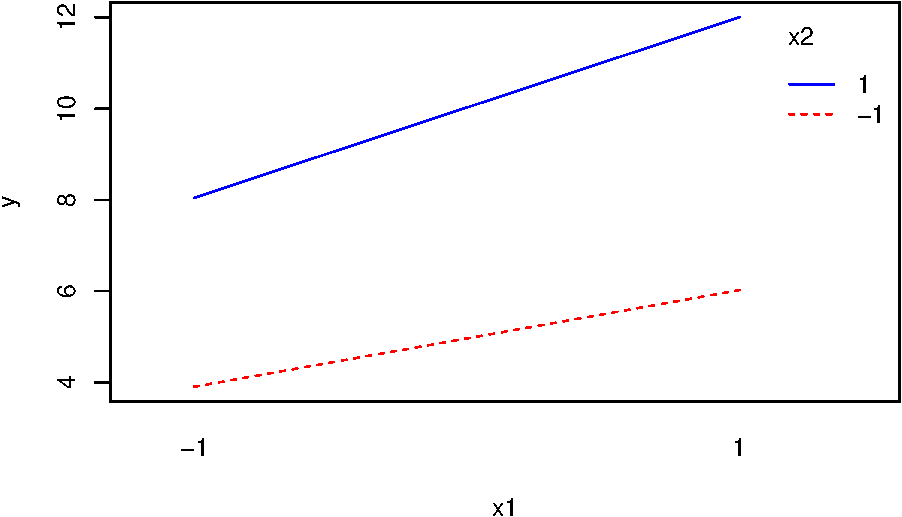
\includegraphics{exercise-interaction_files/figure-latex/unnamed-chunk-1-2.pdf}

\begin{Shaded}
\begin{Highlighting}[]
\NormalTok{b0 }\OtherTok{=}\NormalTok{ interaction.mod}\SpecialCharTok{$}\NormalTok{coefficients[}\DecValTok{1}\NormalTok{]}
\NormalTok{b1 }\OtherTok{=}\NormalTok{ interaction.mod}\SpecialCharTok{$}\NormalTok{coefficients[}\DecValTok{2}\NormalTok{]}
\NormalTok{b2 }\OtherTok{=}\NormalTok{ interaction.mod}\SpecialCharTok{$}\NormalTok{coefficients[}\DecValTok{3}\NormalTok{]}
\NormalTok{b12 }\OtherTok{=}\NormalTok{ interaction.mod}\SpecialCharTok{$}\NormalTok{coefficients[}\DecValTok{4}\NormalTok{]}


\NormalTok{reg.estimates.x1 }\OtherTok{=} \FunctionTok{matrix}\NormalTok{(}\FunctionTok{c}\NormalTok{(b0}\SpecialCharTok{+}\NormalTok{b2,b0,b0}\SpecialCharTok{{-}}\NormalTok{b2,b1}\SpecialCharTok{+}\NormalTok{b12,b1,b1}\SpecialCharTok{{-}}\NormalTok{b12),}\AttributeTok{nrow =} \DecValTok{3}\NormalTok{)}
\FunctionTok{dimnames}\NormalTok{(reg.estimates.x1) }\OtherTok{=} \FunctionTok{list}\NormalTok{(}\FunctionTok{c}\NormalTok{(}\StringTok{"x2=+1"}\NormalTok{,}\StringTok{"x2=0"}\NormalTok{,}\StringTok{"x2={-}1"}\NormalTok{),}\FunctionTok{c}\NormalTok{(}\StringTok{"intercept"}\NormalTok{,}\StringTok{"slope"}\NormalTok{))}

\NormalTok{reg.estimates.x1}
\end{Highlighting}
\end{Shaded}

\begin{verbatim}
##       intercept  slope
## x2=+1    10.024 1.9775
## x2=0      7.496 1.5190
## x2=-1     4.968 1.0605
\end{verbatim}

\begin{Shaded}
\begin{Highlighting}[]
\NormalTok{original.mod }\OtherTok{=} \FunctionTok{lm}\NormalTok{(voltage }\SpecialCharTok{\textasciitilde{}}\NormalTok{ flow}\SpecialCharTok{*}\NormalTok{resistance,}\AttributeTok{data=}\NormalTok{ohms.dat)}
\FunctionTok{summary}\NormalTok{(original.mod)}
\end{Highlighting}
\end{Shaded}

\begin{verbatim}
## 
## Call:
## lm(formula = voltage ~ flow * resistance, data = ohms.dat)
## 
## Residuals:
##       1       2       3       4       5       6       7       8 
## -0.1055  0.1055  0.0365 -0.0365 -0.1125  0.1125 -0.1365  0.1365 
## 
## Coefficients:
##                 Estimate Std. Error t value Pr(>|t|)    
## (Intercept)      -0.8055     0.8432  -0.955 0.393518    
## flow              0.1435     0.1654   0.868 0.434467    
## resistance        0.4710     0.5333   0.883 0.427003    
## flow:resistance   0.9170     0.1046   8.768 0.000933 ***
## ---
## Signif. codes:  0 '***' 0.001 '**' 0.01 '*' 0.05 '.' 0.1 ' ' 1
## 
## Residual standard error: 0.1479 on 4 degrees of freedom
## Multiple R-squared:  0.9988, Adjusted R-squared:  0.9979 
## F-statistic:  1086 on 3 and 4 DF,  p-value: 2.818e-06
\end{verbatim}

\end{document}
